\documentclass[12pt]{article}   	% use "amsart" instead of "article" for AMSLaTeX format
\usepackage{geometry}              		% See geometry.pdf to learn the layout options. There are lots.   
\geometry{
 letterpaper,
 %total={6in, 8in},
 left=20mm,
 top=20mm,
 right=30mm,
 bottom=30mm
 }              		
% this package is to upload graphics 
\usepackage{graphicx}	
% these three packages load some nice math commands
\usepackage{amssymb}
\usepackage{amsthm}
\usepackage{amsmath}

% this package allows to add urls
\usepackage{hyperref}

% this package is for the bibliography
\usepackage{biblatex}
\addbibresource{bibtex.bib}


% this is just a package to generate lipsum text
\usepackage{lipsum}


% Keywords command
\providecommand{\keywords}[1]
{
  \small	
  \textbf{\textit{Keywords---}} #1
}


% this package is to set up double spacing
\usepackage{setspace}


\title{Brief Explanation of Quantum Computing and its Applications}
\author{Gabriel Wies}
\date{\today}		
%\pagestyle{empty}				% Activate to display a given date or no date

\begin{document}
% this will automatically make your title
\maketitle

% you need an abstract for your expository article
\begin{abstract}
Since the conception of computers in the mid $20^{th}$ century, humanity's understanding of the universe and quality of life have improved exponentially. Although the processing power of computers has continued to grow at a fast rate, the limit of what can be achieved with classical computers is becoming more and more evident. In order for humanity to advance to the next level of society, a massive breakthrough must happen in the computational industry. Many experts believe this breakthrough will occur through quantum computing.
\end{abstract}

% you need keywords 3-5 for your expository article
\keywords{superposition, qubit, entanglement, quantum supremacy, quantum computing}

% this creates double spacing
\doublespacing

\section{Limitations of classical computing}
Modern computers can process an immense amount of information and solve extremely complex problems. There is, however, a limit to what even the most powerful supercomputer can solve. Current computers struggle to solve problems such as the factoring of large numbers. This is the primary reason why large prime numbers are used in cryptography. Many optimization problems require a computer to search through trillions of outcome in order to determine the optimal solution. Examples of these optimization problems include simulating the interactions of molecules in the pharmaceutical industry and financial models that minimize risk while maximizing return \cite{1IBM}.\\
There is also an inherent inefficiency to computing. In the case of certain \textit{logic gates}, which require two inputs that comprise of either 0 or 1 and have a single output, information is lost when an output is given. The information of the two inputs is irreversibly lost and result in a dissipation of energy within the system.  Logic gates are not only energy inefficient but also do not conserve information. Whenever a bit of memory is erased in a computer system, we irreversibly lose all information about the previous state of that bit. The inherent inefficiency limits the potential of current computer systems. Another major limitation is that a computational power is limited by the number of bits a system can process. A computer's power grows at a linear rate as the number of bits increase. Computational power has been able to increase exponentially since the conception of modern computers due to the shrinking size of transistors. Current AMD processors have transistors that are 5nm. There is, however, a limit to how small a transistor can get and we are approaching that limit quickly. The only solution to these problems lies within developing a whole new kind of computer that processes information more efficiently \cite{5SCIAMER}. 

\section{Photon polarization and quantum mechanics}
In order to understand how quantum computers work it is important to understand how data can be extracted from quantum particles. Eleanor Rieffel and Wolfgang Polak's book \textit{Quantum computing: a gentle introduction} gives the example of photon polarization in order to explain certain quantum properties. When light interacts with a polarizer, also known as a polaroid, the light waves that pass through are oriented is the same direction as the polaroid. As shown in Figure 1.1, a vertical polarizer will output only vertical waves and the same can be said for a polaroid that is oriented horizontally. While it might seem as if the polaroid is only letting light pass through that is oriented in the same direction as itself, a basic experiment displays that the polarization of photons is dependent on its quantum properties.  \\
\begin{center}
    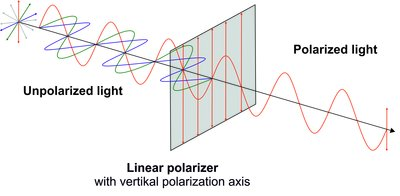
\includegraphics[scale=3]{polaroid2.png}\\
    Figure 1.1: Polaroid outputs waves with the same orientation as itself
\end{center}


When a polaroid is placed between the light and the projection screen the intensity of the light that reaches the screen decreases as shown in Figure 1.2. We call the polaroid with a horizontal polarization polaroid A. We then place polaroid C between polaroid A and the projector screen. As apparent in Figure 1.3, when Polaroid C has a polarization that is perpendicular to that of polaroid A, no light reaches the projector screen.  \\

\begin{center}
    \begin{tabular}{ c c }
 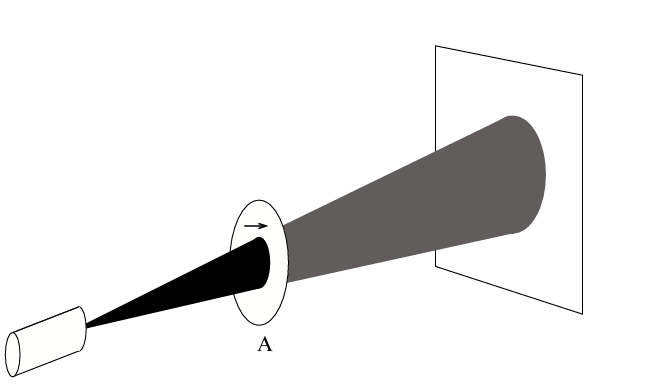
\includegraphics[scale=.5]{fig1.PNG}\label{Figure 1.1} & 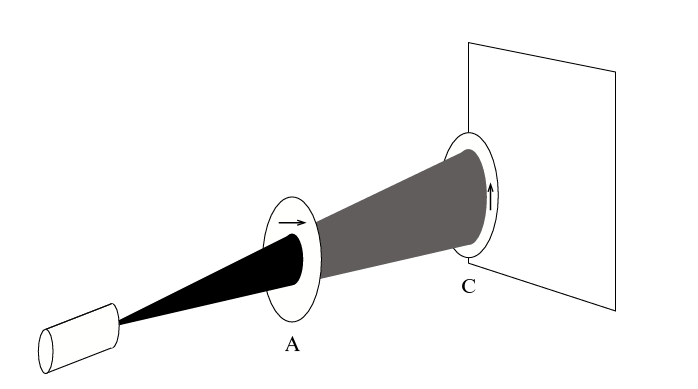
\includegraphics[scale=.5]{fig2.PNG}\label{Figure 1.2}  \\ 
 Figure 1.1: Polaroid A is added & Figure 1.2: Polaroid C is added \\  
\end{tabular}
\end{center}


Next, a third polaroid is placed in between A and B that is oriented with a polarization that is 45$^{\circ}$ between that of A and C. As shown is Figure 1.4 adding a 3rd polaroid make it so light does in fact reach the projector screen. How is it possible that adding a 3rd filter allows light to pass through while having only two did not? Clearly our definition of a polaroid is incorrect and some quantum mechanical process must be happening.\\ 
\begin{center}
    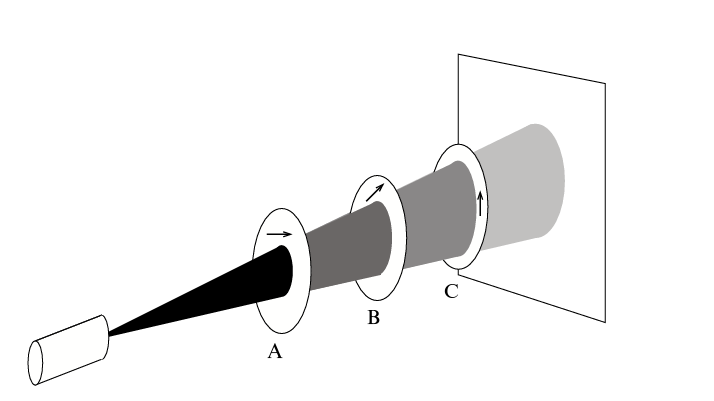
\includegraphics[scale=.5]{fig3.PNG}\label{Figure 1.3}\\Figure 1.3: Polaroid B is added between A and C
\end{center}

The polarization state of a photon is modeled in quantum mechanics by a vector of length $1$, known as a \textit{unit vector}. We can write $|\uparrow\rangle$ and $|\rightarrow \rangle$ as the unit vectors representing vertical and horizontal polarization states respectively. $|v \rangle$ in quantum mechanic represents a arbitrary quantum state. In the previous example we can model polarization as the linear combination $|v \rangle=a|\uparrow\rangle+b|\rightarrow \rangle$ where $a$ and $b$ are the amplitudes of their respective unit vectors. When both $a$ and $b$ are non-zero, $|v \rangle$ is said to be a \textit{superposition} of $|\uparrow\rangle$ and $|\rightarrow \rangle$.\\ 
When a photon with polarization $|v \rangle=a|\uparrow\rangle+b|\rightarrow \rangle$ interacts with a Polaroid with a preferred axis $|\rightarrow \rangle$, the probability that the photon will pass through is equal to $|b|^2$ and the probability that the photon will get absorbed is $|a|^2$. More generally, the probability that a photon passes through is equal to the magnitude of the amplitude of the polarization in the direction of the polaroid.  The photon will also be oriented in the preferred direction of the polaroid if it passes through. \\
In the polaroid experiment, any photon that passes through will be polarized in the horizontal direction, $|\rightarrow \rangle$. The photon now has a no vertical amplitude, $a|\uparrow\rangle=0$. The probability that this photon will be able to pass through a vertically oriented polaroid is 0, $|a|^2=0$. By adding another filter with a preferred axis $|\nearrow \rangle$ between the two, a fraction of the photons that pass through polaroid A will pass through polaroid B and have polarization $|\nearrow \rangle$. $|\nearrow \rangle$ is a superposition of $|\uparrow\rangle$ and $|\rightarrow \rangle$ and therefore there is a probability of $|a|^2$ that the light will pass through polaroid C. The value of $a$ after passing through polaroid B is non-zero so there is a chance that the photon will be able to pass through polaroid C. \\
This polarization example provided by Rieffel and Polak gives  an example of a \textit{quantum bit}, known more commonly as a \textit{qubit}. The space of all possible states of polarization of a photon is an example of a qubit. A qubit value in this case is any state represented by $|v \rangle$. Any system that is quantum-mechanical and that can be modeled by a two dimensional vector space can be viewed as a qubit \cite{2QUANTINTRO}.



\section*{Using qubits for problem solving}
As mentioned in the previous section, qubits exist in a super position of two vector states that are orthogonal to each other. In the polaroid example, the two states $|\uparrow\rangle$ and $|\rightarrow \rangle$ are vectors that are at right angles to each other, also known as orthonormal vectors. In general we interpret these two orthogonal vectors as $|0\rangle$ and $|1 \rangle$. When a qubit is observed, its quantum state immediately collapses to either 0 or 1. Since an observed qubit collapses into one of two states when observed, it can only provide the same amount of data as a classical bit. In order to be computationally superior to conventional computation, qubits are \textit{entangled} into pairs. When two qubits are entangled, the pair exists in a single quantum state. When the state of one of the quibits is changed, the state of the other will simultaneously change in a predictable way. When the amount of bits are doubled in a conventional computer, the processing power of the computer is doubled, while in quantum computers increasing the quibit amount produces an exponential increase in its computational power. Parameters for problems in quantum computing are added by changing the amplitude of the vectors. This means that complex problems can be solved by adding parameters to qubits and entangling them into chains \cite{3MIT}.\\
Complex problems of probability can be solved extremely quickly in this manner through special quantum algorithms that are being developed. In an optimization problem where there are N possible outcomes with only one optimal solution, a conventional computer will have to search through each option individually. On average a classical computer will have to search through $N/2$ items before finding the answer. Using mathematician Lov Grover's quantum search algorithm will yield the result after checking roughly $\sqrt{N}$ outcomes. To put this into perspective, if a problem has 1 trillion possible outcomes with each outcome taking 1 microsecond to check, a classical computer will find the solution in about 1 week. Using Grover's search algorithm on a quantum computer will yield the result in about 1 second \cite{1IBM}.


\section{Current Limitations of Quantum Computing}
The quantum state of qubits is extremely fragile. Even the slightest change in temperature or a vibration can cause the qubits to fall out of superposition. This loss of information is called decoherence. As a result current quantum computers super cool their qubits to near absolute zero and maintain a vacuum. Despite these precautions external noise still causes errors in calculations. Quantum algorithms are being developed  in order to compensate for errors due to decoherence. Adding more qubits also helps with reliability. It is predicted that it will take thousands of qubits in order to form a highly reliable "logical" qubit. IBM's largest current quantum computer contains only 65 qubits with the plan of building one that contains 127 qubits by the end of 2021. There is still a long way to go in quantum computer research before any advanced calculations can be achieved. Google has plans to build a million qubit quantum computer in the next ten years. They also have claimed that they already have achieved quantum supremacy, the event where a quantum computer is capable of solving problems that would overwhelm any conventional computer. Google's current claim about achieving quantum supremacy with their 53 qubit system has been heavily contested with many saying the problem could be solved with current conventional computational powers. While there are disagreements about the capabilities of current quantum computers, no one disagrees that quantum supremacy will be achieved very soon, elevating humanity into the next level of civilization \cite{4SCIMAG}. 


\printbibliography

\end{document}  